\chapter[\hspace{0pt}绪\hskip\ccwd{}论]{{\heiti\zihao{3}\hspace{0pt}绪\hskip\ccwd{}论}}\label{chapter: 绪论}

本章内容共分为四节,\hyperref[section1: 研究背景及意义]{第一节}介绍本文的研究背景及意义;\hyperref[section1: 国内外研究现状与挑战]{第二节}总结医学病理图像领域及视觉Mamba的国内外研究现状,并对其面临的挑战进行分析;\hyperref[section1: 本文研究内容与创新点]{第三节}介绍本文的研究内容与创新点;\hyperref[section1: 本文组织结构]{第四节}对本文组织结构进行概括。

\section[\hspace{-2pt}研究背景及意义]{{\heiti\zihao{-3} \hspace{-8pt}研究背景及意义}}\label{section1: 研究背景及意义}


随着全球人口老龄化进程的不断加速,以及疾病发生率呈现显著增长趋势,临床医学领域对精准高效的疾病诊断技术需求日益凸显。
依据《“健康中国 2030” 规划纲要》~\cite{HealthyChina2030},我国人口老龄化进程加快,慢性疾病负担日益沉重,这无疑对医疗诊断的准确性与效率提出了更高要求。
%以癌症为例,据统计,2022年,全球新发癌症病例为1996万,癌症死亡数为974万;我国的情况同样严重,2022年新发病例:482.47万,癌症死亡人数为257万。如此众多的患病人数,给全球的医疗领域都带来了极大冲击。而诊断是治疗的前提,提高疾病诊断的效率与精度的需求刻不容缓。\cite{krizhevsky2012imagenet, yolo, FasterRcnn, MaskRcnn, 图像分类, 陈科圻2020多尺度目标检测的深度学习研究综述, 蒋弘毅2021目标检测模型及其优化方法综述, 语义分割},在某些特定任务中的表现达到甚至超越了人类的水平。然而,这些技术的成功在很大程度上依赖于大规模标注数据集的支撑。一旦没有足够数量的标注样本,很多深度学习模型便会因为只在少量样本数据上进行训练而出现过拟合或欠拟合现象,进而导致无法达到良好的性能表现。
病理诊断作为疾病诊断的 “金标准”,在临床决策中占据关键地位~\cite{pinckaers2020streaming,lu2021ai,侯乃侨2024显微知著}。而传统依靠病理医生在显微镜下人工阅片的方式存在明显短板。
如在病理诊断实践中,细胞与组织形态学的显著异质性特征以及肿瘤表型的微小异质性差异,共同构成了该领域的核心挑战。这种复杂性要求病理医师不仅需要具备深厚的专业知识储备,更依赖于长期临床实践经验的支撑。
然而,病理医师培养周期长且成本高昂的现状,与临床需求之间的矛盾日益凸显。
同时,视觉观察的主观性叠加切片染色过程中产生的颜色偏差与形态差异,可能导致诊断结果的不一致性,甚至引发误判。
此外,高分辨率病理图像通常包含亿级像素信息,而病灶区域仅占图像面积的极小比例(如图~\ref{figure1: WSI图像肿瘤区域示意图})病理医师需在有限时间内完成大量图像的精读分析,显著降低了人工诊断的效率与准确性。

\begin{figure}[h]
    \centering
    \captionsetup{font={small, stretch=1.312}}
    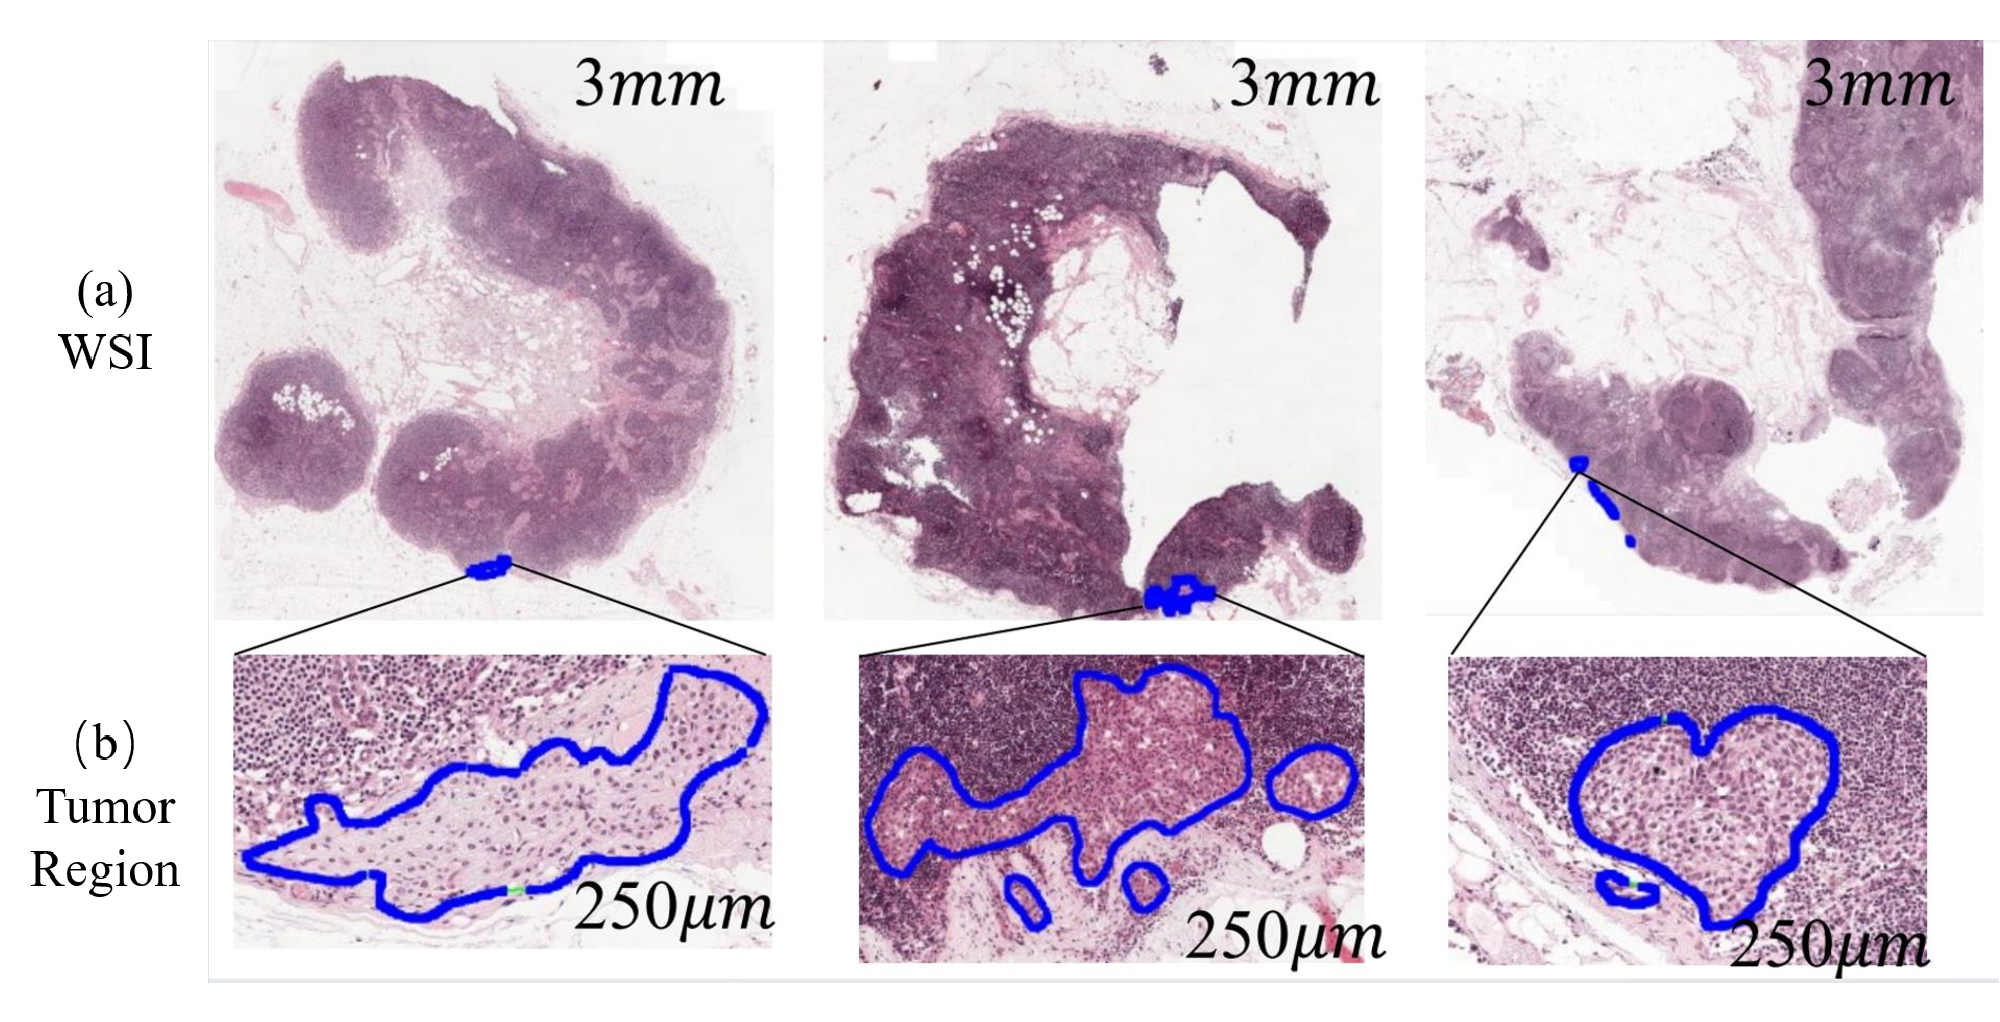
\includegraphics[width=1.0\columnwidth]{figures/fig1.pdf}
    \bicaption[Camelyon16数据集中肿瘤区域相对于正常区域的比例示例图]{Camelyon16数据集中肿瘤区域相对于正常区域的比例示例图。}[Example of the proportion of the tumor region to the normal region in the Camelyon16 dataset]{Example of the proportion of the tumor region to the normal region in the Camelyon16 dataset.}
    \label{figure1: WSI图像肿瘤区域示意图}
\end{figure}
与此同时,随着人工智能在各领域的蓬勃发展,AI赋能医疗给病理智能诊断提供了可能。国务院印发的《新一代人工智能发展规划》~\cite{NewGenAIDevPlan}着重指出,要加速人工智能在医疗领域的应用,全力推动医疗影像辅助判读等技术的进步。
利用高分辨率数字病理扫描仪通过高效精准的数字化流程,可以将组织切片转换为亿级像素的全幅切片图像(Whole Slide Image, 下文简称病理图像或WSI)~\cite{唐仲平2018全切片图像扫描技术在临床病理诊断工作中的应用},
而这些图像便于存储、传输与共享,打破了时空限制。加之计算机视觉技术的突飞猛进,图像处理、人工智能及机器学习算法持续创新,让病理图像自动化分析从设想走向现实。通过对海量数字病理图像的深度学习,计算机模型有能力捕捉到人类肉眼难以察觉的病变特征,以提高病理诊断的效率与准确性。

然而,针对如此高分辨的WSI图像而言,传统深度学习算法仍有不小挑战:数十亿像素的图片如直接输入到传统的分类器中,将导致难以承担的计算成本;
而若采用采样出的低分辨率的缩略图作为输入,则会不可避免的丢失大量关键信息,造成性能上的损失。
同时,由于病理图像的标注需要大量专家知识,因此细粒度的图像标注过程既耗时又耗力。当前,在仅提供低精度标注的场景下,如何充分挖掘未标注数据的潜力以优化模型效能,已成为数字病理图像分析领域的核心研究方向之一。
\begin{figure}[h]
    \centering
    \captionsetup{font={small, stretch=1.312}}
    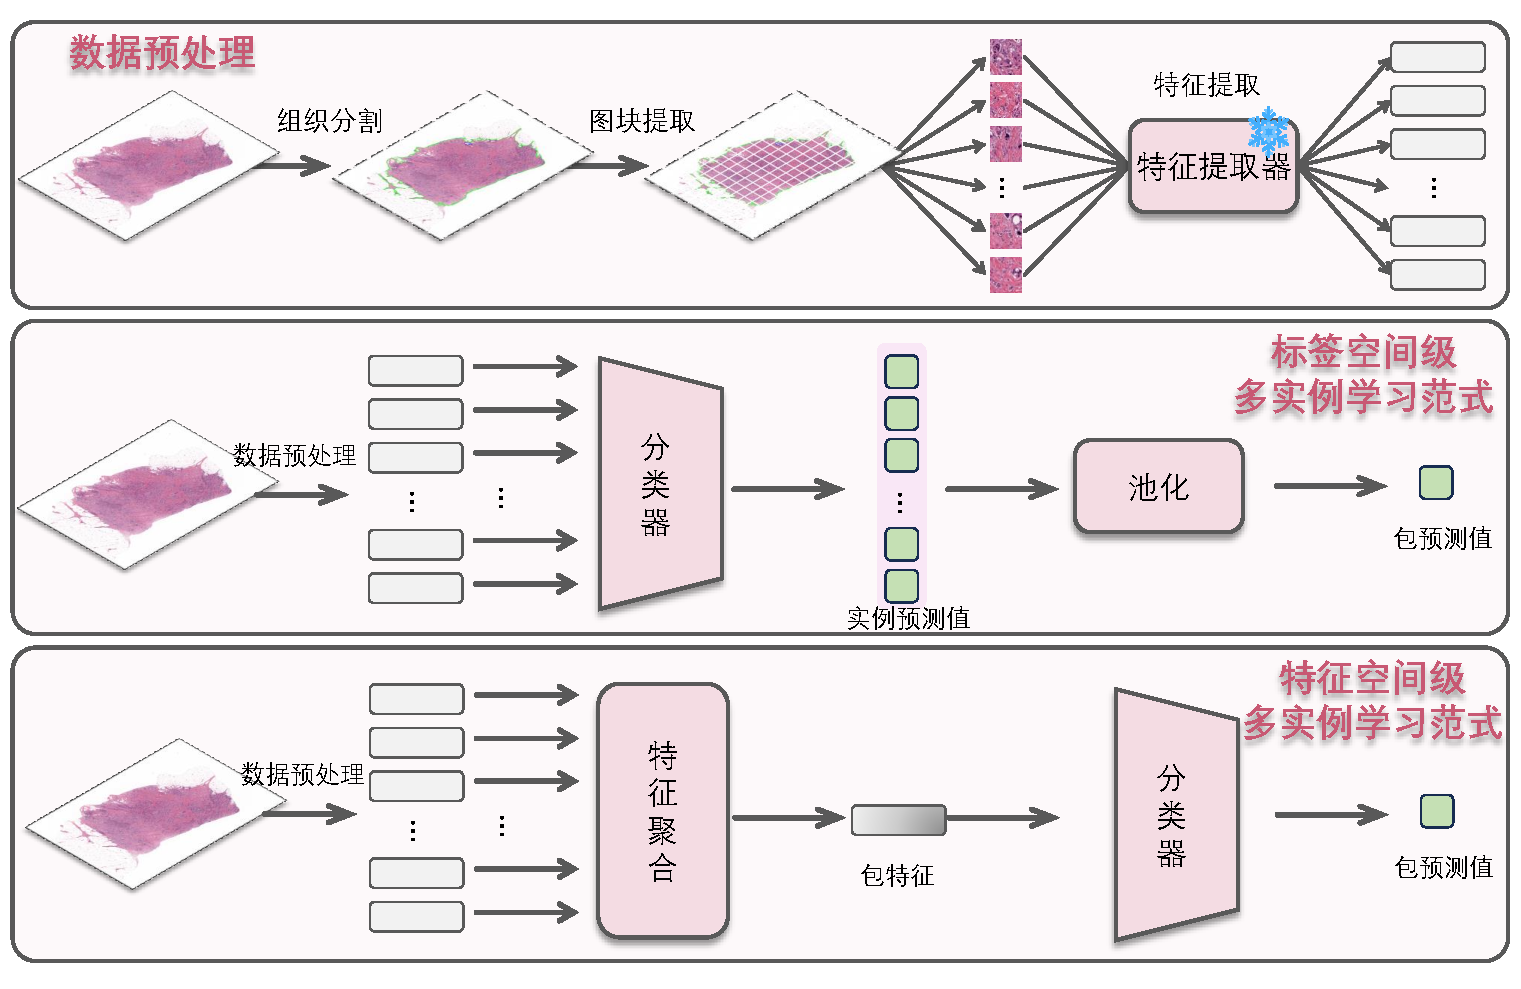
\includegraphics[width=\columnwidth]{figures/多实例学习范式.pdf}
    \bicaption[两种多实例学习范式示意图]{两种多实例学习范式示意图。}[The illustration of two paradigms for multiple instance learning.]{The illustration of two paradigms for multiple instance learning.}
    \label{figure1: 多实例学习范式}
\end{figure}

多实例学习(Multiple Instance Learning,MIL)\cite{dietterich1997solving,herrera2016multiple}作为一种特殊的弱监督学习框架是业内解决这一类问题的常见技术手段~。
具体而言,每张病理图像都被视为一个“包”(Bag),并会被进一步分割成大量图块(Patch),这些图块被定义为“包”中的“实例”(Instance)。
其目标是在分类标签(如“恶性”或“良性”)作用于整个包的情况下,通过分析实例与包标签之间的关联性,挖掘出关键实例特征,并基于这些信息完成对整张图像的分类。
然而,在病理图像的实际应用场景中,多实例学习框架虽然得到了广泛应用~\cite{li2021dual,lu2021data,shao2021transmil,zhang2022dtfd,tang2024feature},但仍然面临着诸多现实问题。
由于尺寸巨大,切分后的实例数目众多,导致在使用具有较强建模能力的传统ViT~\cite{dosovitskiy2020image}进行实例处理时所需的计算资源消耗巨大,只能采取减少实例数目或更换为线性注意力机制的折中方案。

而近期,一些基于状态空间模型(State Space Model,SSM)~\cite{hamilton1994state}的架构为解决上述问题,提供了新的思路。
Mamba~\cite{gu2023mamba,mamba2}是最近提出的一种具有代表性的基于SSM架构的模型,与ViT相比具有更好的长序列建模能力,而且仅需线性的计算资源。
自从其引入到视觉领域后,在分类~\cite{zhu2024vision,yue2024medmamba,DATE20250218001,yao2024spectralmamba}、检测~\cite{BJHK20241114002,ZGGL202412016,chen2024mim,zhang2025cdmamba}、
分割~\cite{GXXB20250212011,JSGG20240822004,li2025selective,wu2025h}等任务中已经取得了显著的表现,展现出了宏大的应用前景。
然而作为原本被提出解决序列问题的Mamba总是倾向于建模出一种前序Token与后序Token的因果关系,
这与病理图像多实例学习的序列不变特性并不相符~\cite{huang2024localmamba}。并且,其以一维序列作为输入,常常无法完全捕获图像中的二维空间信息。
鉴于此,针对高分辨率数字病理图像分类任务,通过构建基于 Mamba 的模型框架弥合序列相关的 Mamba 模型与序列无关的 WSI 分类任务之间的性能差异,深度挖掘病理图像的空间特征信息,进而优化模型的分类效能,推动数字病理图像计算机辅助诊断准确率的显著提升,具有重要的临床应用价值与学术研究意义。

\section[\hspace{-2pt}国内外研究现状与挑战]{{\heiti\zihao{-3} \hspace{-8pt}国内外研究现状与挑战}}\label{section1: 国内外研究现状与挑战}

\subsection[\hspace{-2pt}数字病理图像分类研究现状]{{\heiti\zihao{4} \hspace{-8pt}数字病理图像分类研究现状}}\label{section1: 数字病理图像分类研究现状}

鉴于数字病理图像分辨率极高,同时细粒度像素级标注较为匮乏,当前研究工作普遍借助多实例学习框架攻克数字病理图像的分类难题。
多实例学习,英文表述为 Multiple Instance Learning,简称为 MIL,部分文献也将其译为多示例学习。
多实例学习的经典范式最早由 Dietterich TG 等学者于 1997 年在药物活性预测研究中首次提出并成功应用~\cite{dietterich1997solving}。
作为弱监督学习领域的典型框架,该技术已受到学术界的广泛关注。其训练数据通常由带有类别标签的包集合构成,每个包内包含多个未标注实例,构成独特的弱监督学习模式。
正包中至少含有一个正实例,负包中只包含负实例。
在多实例学习的训练过程中,只需要提供粗粒度的包级标签(如病人是否患癌),而在实际场景中粗粒度的包级标签往往是易获取的,
从而使得多实例学习非常契合多种实际场景,很多问题可以自然的表述为多实例问题。
以药物活性预测问题为例~\cite{dietterich1997solving},在该问题里,主要的任务目标在于对某一种新分子是否适宜用于制药进行预测。实际情况是,每一个分子都存在着多种可能的低能形状。
所获得的标签信息仅仅是明确了哪些分子是适合制药的,然而对于究竟是分子的哪一种具体低能形状在其是否适合制药这一判定中起到了关键决定性作用,却并不清楚。
鉴于这样的情况,在处理该问题时,便将每一个分子当作是一个 “包”,而分子的每一种低能形状则对应成为这个 “包” 中的一个 “实例”,如此一来,就形成了多实例学习中所定义的实例与包的关系模式。
由于其独有的特性,多实例学习在各个领域都得到了广泛的发展和应用,如目标检测~\cite{hoffman2015detector,wu2015deep,陈钰2016基于,tang2018weakly},语义分割~\cite{xu2019camel},
图像和视频分类~\cite{唐大伟2014壁画图像分类中的分组多实例学习方法,huang2021weakly,wang2013max,chen2006miles,rahmani2006missl,andrews2002support},文本分类~\cite{zhou2009multi},医学图像分类~\cite{ilse2018attention,shao2021transmil,zhang2022dtfd,kanavati2020weakly,li2021dual,chikontwe2020multiple}等。

当前,多实例学习方法主要分为标签空间方法与特征空间方法。标签空间方法基于实例级标签推断聚合策略直接预测包标签,其实例间关系建模能力有限,且在大规模数据集中面临计算效率瓶颈~\cite{campanella2019clinical}。
鉴于此,当前研究重点逐渐转向特征空间方法,这类方法通过整合包内所有实例的特征信息,构建包的嵌入特征表示,进而实现包级标签的预测。
例如,Ilse等人~\cite{ilse2018attention}提出的AB-MIL,在多实例学习框架中引入基于注意力的聚合层,通过神经网络以参数化方式量化每个实例对于包级特征嵌入的贡献。
Li 等学者~\cite{li2021dual}在研究中提出并构建了 DSMIL 方法,通过融合自监督对比学习与金字塔特征融合机制高效提取实例级特征,并创新性地引入非局部注意力模块聚合多尺度实例信息,从而显著提高 WSI 全切片图像分类任务的准确率。
DTFD-MIL~\cite{zhang2022dtfd}引入双层多实例学习框架,将图像分割成多个伪包,通过聚合伪包的预测结果,推断整个病理图像的标签。Zhu等人~\cite{zhu2024dgr}提出DGR-MIL模型,通过引入可学习的全局向量,精准识别最具代表性的实例,并采用交叉注意力机制计算实例间的重要性,有效挖掘病理图像中的关键特征。Shao等人~\cite{shao2021transmil}将Transformer架构引入多实例学习框架中,利用空间位置编码保留空间拓扑结构,并通过注意力机制实现实例间关系的多粒度建模。

Transformer中自注意力机制计算成本高昂,限制了其在大规模图像数据处理任务中的推广与应用。因此,Tang等人~\cite{tang2024feature}通过将病理图像划分为多个区域,显著减少Token数量,并引入线性自注意力机制,降低计算成本的同时有效建模实例间的关系。
然而,这种轻量型的自注意力机制会在一定程度上削弱模型对复杂实例关系的建模能力。
最近提出的Mamba模型~\cite{gu2023mamba}因其高效的计算效率和强大的实例关系建模能力成为了热门模型,
但作为与输入顺序相关的序列模型,Mamba对实例扫描模式非常敏感,这与多实例学习对序列不变性的要求相冲突,
影响了其在病理图像分类任务中的稳定性,限制了其在病理图像分类中的潜力。


\subsection[\hspace{-2pt}视觉Mamba研究现状]{{\heiti\zihao{4} \hspace{-8pt}视觉Mamba研究现状}}\label{section1: 视觉Mamba研究现状}

Mamba最初是在自然语言处理领域提出的,作为一种更有效地处理长序列的架构\cite{gu2023mamba}。
与Transformer \cite{vaswani2017attention}等传统模型不同,Mamba采用了一种选择性状态空间模型(SSM \cite{kalman1960new}),该模型基于内容动态地过滤和处理信息,使模型能够选择性地记住或忽略部分输入。
Mamba在处理速度和可扩展性方面提供了显著的改进,特别是对于较长的序列。
Zhu等人首先将Mamba引入视觉领域研究人员们的视野\cite{zhu2024vision},其在具有强大的建模能力的同时仅需线性计算资源的特点,让其迅速在分类、检测、分割等诸多领域取得令人惊奇的效果。
\begin{figure}[h]
    \centering
    \captionsetup{font={small, stretch=1.312}}
    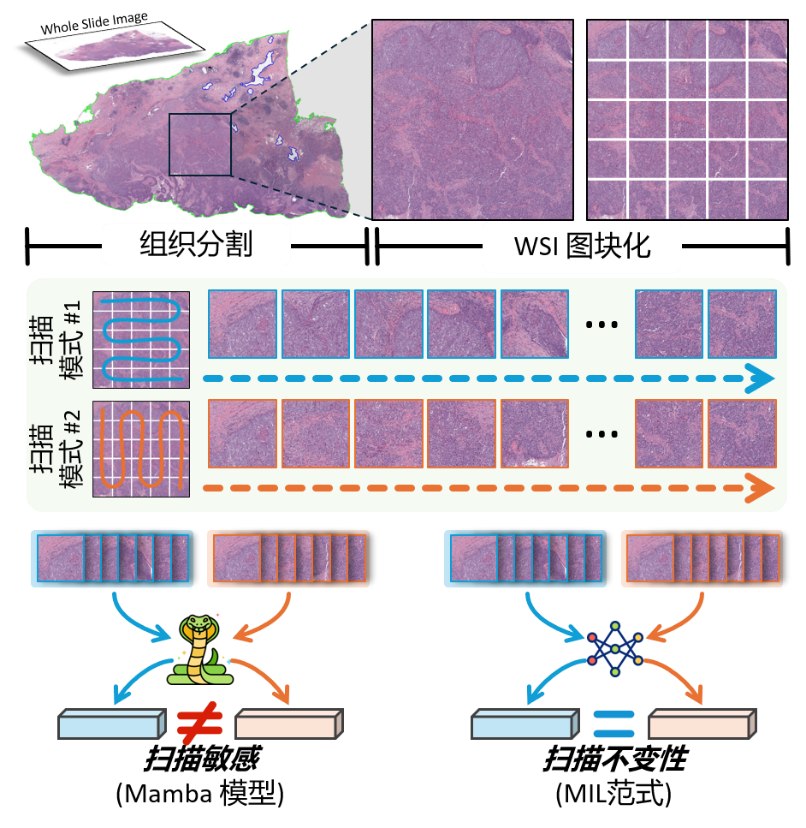
\includegraphics[width=0.7\columnwidth]{figures/Discrepancy1.png}
    \bicaption[Mamba模型与MIL任务差异图]{Mamba模型与MIL任务差异示意图。}[Discrepancy between Mamba and MIL for computational pathology tasks]{Discrepancy between Mamba and MIL for computational pathology tasks.}
    \label{figure1: Mamba模型与MIL任务差异}
\end{figure}

然而,Mamba作为一种自回归模型,在视觉任务与多实例学习任务中固有地表现出差异,如图\ref{figure1: Mamba模型与MIL任务差异}所示:Mamba假设之前和之后的斑块之间存在因果关系\cite{liu2024vmamba},
而在图像中,不同斑块之间不存在这种因果关系,甚至在多实例学习范式中更是将各个实例视为“平等”实例,并无顺序关联。因此,许多研究通过聚合多种扫描模式来减轻Mamba对序列顺序的敏感性。例如,Vim\cite{zhu2024vision}通过组合来自两个分支(向前和向后)的结果来减轻序列顺序的影响。而Vmamba\cite{liu2024vmamba}采用了四种扫描模式:左上到右下、右下到左上、右上到左下、左下到右上。这些模式综合多个信息序列以提高性能。 LocalMamba~\cite{huang2024localmamba}引入了一种新的局部扫描策略,将图像划分为不同的窗口,综合横向、纵向、局部等多种扫描模式,在保持全局视角的同时有效地捕获局部依赖,大大提高捕获有效图像表示方面的性能。

对于病理图像分类而言,MamMIL\cite{fang2024mammil}结合了Bi-SSM和2D-CAB模块,整合了来自原始、反向和局部序列的扫描模式信息,从而增强了WSI分类。
此外,MambaMIL\cite{yang2024mambamil}将序列重塑成一个矩形,并应用序列重排序操作来垂直扫描新序列,提高了其模拟长序列的能力。
然而,这些方法过度关注输出序列信息的整合,未能从根本上突破序列输入顺序对Mamba建模能力的约束,仅仅是一种妥协的策略,其依旧高度依赖扫描模式和集成形式,使得模型性能不够稳定性。

\section[\hspace{-2pt}本文研究内容与创新点]{{\heiti\zihao{-3} \hspace{-8pt}本文研究内容与创新点}}\label{section1: 本文研究内容与创新点}

本文研究了Mamba架构在病理图像分类中的应用。
虽然Mamba架构在处理病理图像分类任务时,可以解决由于实例数目过多导致的问题,例如计算资源消耗巨大、实例间关系建模不充分等,
但其仍然存在其无法捕获二维空间关系、以及与病理图像多实例学习的序列不变性存在冲突等问题,与病理图像分类任务并不完全适配。
如何缓解甚至消除二者其中的差异依旧是将高效且性能卓越的Mamba架构适配到病理图像领域一个重要的且有挑战性的问题。
因此,本文研究了Mamba架构在病理图像分类中的应用,分别从多扫描模式融合Mamba和扫描不变性Mamba的两个角度开展以下研究:

\textbf{(1)基于多扫描Mamba的高分辨率病理图像分类研究}

针对Mamba一维序列建模所造成图像空间结构捕获能力不足的问题,
本文从Mamba整合多种扫描模式的角度出发,提出基于空间信息增强实现的多扫描Mamba的多实例学习框架(\textbf{M}ulti-scan \textbf{M}amba with \textbf{S}patial information enhancement ,简称M$^2$S-MIL)。
由于常用扫描模式未关注到图像的局部连续性、旋转不变性等特性,该框架采用了多个扫描模式分支作为Mamba的输入,通过设计了区域螺旋扫描和网格扫描等新的扫描模式,
提高Mamba对局部连续性、旋转不变性以及同一序列不同方向的空间关联信息的捕获能力。同时为进一步提升序列的2D空间上下文的感知能力,设计了基于分块局部注意力的2D空间上下文感知模块,
利用区域内的信息整合更进一步提高Mamba对空间能力的捕捉,使Mamba模型更适配于病理图像分类任务。
在3个WSI分析子任务和7个数据集上的大量实验表明,综合多种扫描模式分支,引入空间信息,
能够切实解决Mamba从一维实例序列中空间建模不充分的问题,显著提高模型性能,同时在数字病理图像分类任务中一定程度缓解了使用Mamba模型出现的建模倾向差异难题。​

\textbf{(2)基于扫描不变性Mamba的高分辨率病理图像分类研究}

%利用多扫描模式的信息融合缓解Mamba建模能力与病理图像任务间差异的想法是直截了当的,
%然而这种方法没有本质上突破输入秩序对Mamba建模能力的约束,仅是一种妥协式的策略。
%因此,
本文针对Mamba作为序列相关模型,与病理图像多实例学习的序列不变性存在冲突的问题,从构建扫描不变性Mamba角度出发,提出了基于对比学习策略实现的扫描不变Mamba的多实例学习(\textbf{S}can-invariant \textbf{M}amba with \textbf{C}ontrastive Learning ,简称SMC-MIL)框架。
为了指导 Mamba 学习到不同实例扫描序列中一致的包特征,本文设计了双分支实例序列对比学习框架,通过约束同一Mamba从不同扫描序列获得的包表示及分类结果保持一致,来引导Mamba学习与序列顺序无关的特征。
同时引入基于实例评估的序列对比增强方法,来增加对比学习难度,迫使Mamba在输入序列差异极大的情况下,
学习到对病理图像形成一致表示和决策的能力,成功赋予Mamba良好的序列不变建模和实例识别能力。
实验结果显示,SMC-MIL在继承了Mamba优异计算效率和建模能力的同时,有效降低模型对输入序列顺序的敏感性,
专注于实例无序关系建模,挖掘出更具显著性判别特征的实例,更好地适配病理图像分类任务。

本文提出的M$^2$S-MIL模型与SMC-MIL模型分别从多扫描模式Mamba和扫描不变性Mamba的两个角度出发,对数字病理图像分类任务中Mamba的应用进行深入的剖析和研究。
M$^2$S-MIL模型通过综合多种扫描模式的特征信息,并引入空间上下文感知模块,进一步提升Mamba对2D空间信息的捕获能力,缓解原本一维Mamba模型对2D病理图像空间建模能力不足的问题;
SMC-MIL模型则进一步突破扫描顺序对Mamba建模能力的约束,弥合了原本Mamba的序列敏感性与病理图像多实例学习中序列不变性假设的冲突,
使Mamba架构更加适配病理图像分类任务,并提高了模型挖掘更具判别性区域的能力,从而提升模型性能。

图~\ref{figure1: 主要研究内容}展示了本文的主要研究内容和贡献。

\begin{figure}[h]
    \centering
    \captionsetup{font={small, stretch=1.312}}
    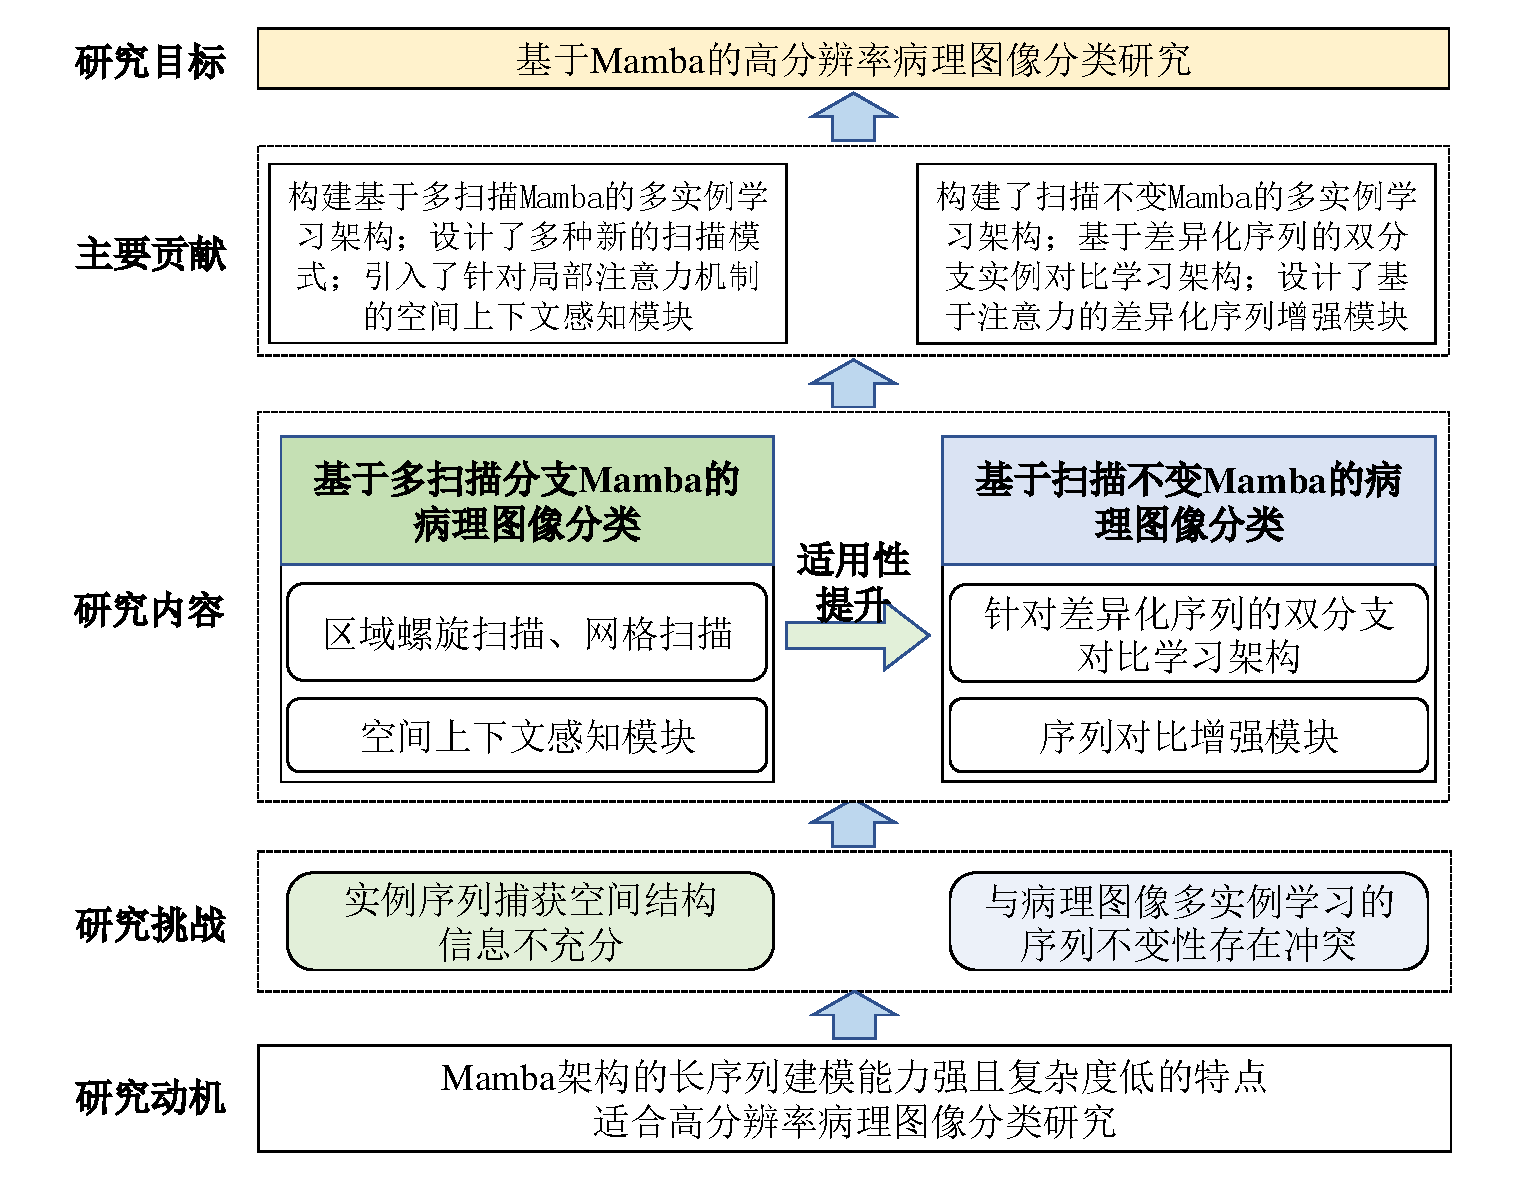
\includegraphics[width=1.0\columnwidth]{figures/研究内容.pdf}
    \bicaption[本文的主要研究内容图]{本文的主要研究内容。}[The main research content of this paper]{The main research content of this paper.}
    \label{figure1: 主要研究内容}
\end{figure}

\section[\hspace{-2pt}本文组织结构]{{\heiti\zihao{-3} \hspace{-8pt}本文的组织结构}}\label{section1: 本文组织结构}

本文由 5 个章节构成,从多个维度深入探讨基于 Mamba 的高分辨率数字病理图像分类研究。下面为各章节的具体介绍:

第一章:绪论。本章首先阐述高分辨率数字病理图像分类任务的研究背景与科学意义,在系统梳理国内外前沿研究进展的基础上,重点剖析基于视觉 Mamba 架构的数字病理图像分类技术现状及存在的挑战。最后对本文的研究内容和组织结构进行概述。

第二章:相关研究技术与理论。首先系统阐述本课题涉及的基础理论框架,涵盖病理图像多实例学习范式、Mamba 模型架构原理及对比学习机制等核心内容。在此基础上,详细解析所用实验数据集、性能评估指标体系及数字病理图像预处理技术路线。

第三章:基于多扫描融合Mamba的高分辨率医学病理图像分类研究。
首先,通过深入剖析现有 Mamba 病理图像分类算法在空间结构建模能力方面的局限性,提出了基于多扫描Mamba的高分辨率病理图像分类算法(M$^2$S-MIL),最后通过在3个WSI任务和7个数据集上的大量实验证明了M$^2$S-MIL模型的有效性。

第四章:基于扫描不变性Mamba的高分辨率医学病理图像分类研究。首先对基于多扫描序列融合Mamba的病理图像分类算法的不足进行分析介绍,提出了基于扫描不变性不变性Mamba的病理图像分类算法(SMC-MIL),然后介绍了提出的SMC-MIL模型的模型框架以及其中的双分支实例序列对比学习框架和序列对比增强模块,并通过系统的实验验证SMC-MIL模型充分赋予了Mamba扫描不变属性。

第五章:总结与未来展望。总结并分析了本文提出的基于Mamba的高分辨率病理图像分类算法研究的成果及不足,并对未来的研究方向与内容进行了展望。

